
\chapter{Graph Matching}

In this chapter we review basic definitions and notations from the graph theory used in this thesis and introduce different forms and formulations of the graph matching problem together with some algorithms for solving them. The classification we use is based on~\cite{Conte2004}, although we concentrated our attention mainly on one specific group of algorithms: those, which consider the graph matching problem as a quadratic optimization problem. Not all algorithms, we present thereby, were initially mentioned in~\cite{Conte2004}, but we also do not cover all of the resent ones due to their quantity. We focus our selfs specially on those, that are important for further reading of the thesis.

\section{Basic definitions and notation}
A \emph{undirected graph} $G=(V,E)$ is defined as a pair of disjoint sets $V$, $E$, where $E\subseteq\{\{u,v\}| u, v\in V\}$~\cite{Diestel2000}. The elements of the set $V$ are called \emph{vertices} or \emph{nodes}\footnote{We use terms vertex and node further in the text as synonyms} and the elements of $E$ are called \emph{edges}. Where it is necessary, we will write $V(G), E(G)$ to refer node and edge sets to the graph $G$.

The number of nodes in $V$ defines the \emph{size} of a graph $G$.
Two nodes $v_{i},v_{i'}\in V$ are called \emph{adjacent}, if there is an edge $e=\{v_{i},v_{i'}\}\in E$. Each graph can be represented by its \emph{adjacency matrix A=$(a_{ij})_{n\times n}$}, where 
\begin{equation*}\centering
a_{ij}=\begin{cases}
 1, & \text{if } \{v_{i},v_{i'}\}\in E, \\
 0, & \text{otherwise.} \\
\end{cases}
\end{equation*}
and $n$ is the number of nodes in the graph.

A \emph{path} in a graph $G=(V,E)$ is a sequence of nodes $\{v_0,v_1,\dots,v_k\}$ connected by the edges $\{v_0v_1,v_1v_2,\dots,v_{k-1}v_k\}$, where $v_i\in V$ and $v_{i-1}v_i\in E$ for all $i=0,\dots,k$. A path with $v_0=v_k$ is a \emph{cycle}.

A graph $G'=(V',E')$ is called a \emph{subgraph} of a graph $G=(V,E)$, if $V'\subseteq V$ and $E'\subseteq E$. We use the standard notation $G'\subseteq G$ for this. The subgraph $G'$ of $G$ is \emph{induced by the set $V'\subseteq V$}, if $E'=\{(v_i, v_{i'})|v_i,v_{i'}\in V'\}$. Analog, the set $E'\subseteq E$ induces the subgraph $G'$ of $G$, if $V'=\{v\in V|v\in e\text{ and }e\in E'\}$. For the induced subgraph we use the notation $G'=G[V']$ and $G'=G[E']$~\cite{Diestel2000}, depending if it is node- or vertex-induced. We also define graph cut $G\cap G'=(V\cap V', E\cap E')$ and union $G\cup G'=(V\cup V', E\cup E')$.

There are several special types of graphs. A graph, whose each pair of nodes is connected by an edge is called \emph{complete}. In case, when each node $v_i\in V$ of a graph $G$ has an associated attribute $d_i\in D$, one speaks about \emph{attributed graph} $G=(V,E,D)$. If in contract to this each edge of a graph has an associated weight, the graph is called \emph{weighted graph}. A connected, undirected graph without cycles is called a \emph{tree}. A $hypergraph$ is graph, whose edges connect several vertices at the same time (\emph{hyperedges}).

Consider two undirected attributed graphs $G^I = (V^I, E^I, D^I)$ and $G^J = (V^J, E^J,\newline D^J)$. We assume the situation, where $|V^I|=n_1$, $|V^J|=n_2$ and $n_1\le n_2$. A \emph{matching function} between $G^I$ and $G^J$ is a mapping $m:V^I\rightarrow V^J$ between the sets of nodes of two graphs.
It is clear, that defined in this way the mapping $m$ is not unique. Assume, that we have some metric $S(G^I, G^J, m)$ to measure the quality of matching $m$. In this case, \emph{Graph matching problem} between $G^I$ and $G^J$ can be defined as a problem of finding such a map $m:V^I\rightarrow V^J$, that maximizes the similarity score $S(G^I, G^J, m)$ between the graphs and fulfills some additional constraints:
\begin{equation} \label{gGMP}
m = \argmax_{\hat{m}}S(G^I, G^J, \hat{m})
\end{equation}
Based on the required properties of the mapping $m$ the algorithms, that solve this problem, can be divided into two large groups~\cite{Conte2004}: \emph{exact} and \emph{inexact} graph matching methods. There are also variations inside of each group based on the definition of the similarity score between two graphs. In the following sections we will give an overview of the common exact and inexact graph matching algorithms.
 
\section{Exact graph matching}
The group of exact graph matching algorithms represents a class of more strict methods, that require the mapping between nodes of two graphs to be \emph{edge preserving}. With other words: if $\{v_i,v_{i'}\}\in E^I$, then $\{m(v),m(v_{i'})\}\in E^J$ for all $v_i,v_{i'}\in V^I$. The graphs, considered in this case often do not have attributes.

There are several forms of the exact graph matching. The most known one is \emph{graph isomorphism}: two graphs are called \emph{isomorph} ($G^I\simeq G^J$), if the edge preserving mapping between their nodes is bijective. This implies, that two graphs have the equal number of nodes. If it is not the case, and the isomorphism holds between the one graph and a node-induced subgraph of the other graphs, the problem is called \emph{subgraph isomorphism}. Its further extension is a isomorphism between subgraphs of the graphs. The last problem can obviously have several solutions, but one is normally interested in finding a common subgraph with maximum number of nodes or edges (\emph{maximum common subgraphs}).  

The further simplification of the graph isomorphism is to require an injective edge-preserving mapping, instead of bijective. This problem is called \emph{graph monomorphism}. The correspondences here are still one-to-one, but the second graph may contain additional nodes and edges, comparing to the first graph.
Even weaker form of graph matching problem is \emph{graph homomorphism}. It allows many-to-one mapping between nodes of two graphs, which means that the only one restriction on the mapping $m$ is to be total.
On the Fig.~\ref{fig:Exact_GM} one can see examples of different exact graph matching problems.
\begin{figure}[h!]
    \centering
    \begin{subfigure}[b]{0.3\textwidth}
        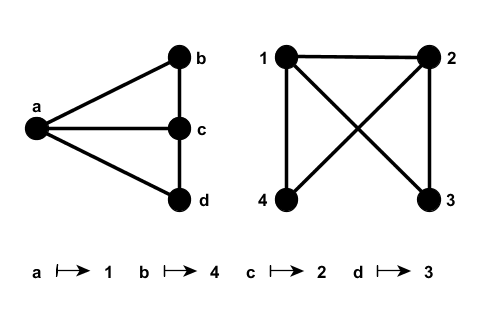
\includegraphics[width=\textwidth]{chapter1/fig/GI}
        \caption{Graph isomorphism}
        \label{fig:GI}
    \end{subfigure}
    ~
    \begin{subfigure}[b]{0.3\textwidth}
        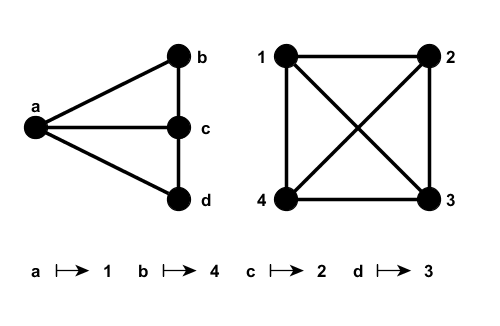
\includegraphics[width=\textwidth]{chapter1/fig/monomorphism}
        \caption{Graph monomorphism}
        \label{fig:monomorphism}
    \end{subfigure}
    ~
    \begin{subfigure}[b]{0.3\textwidth}
        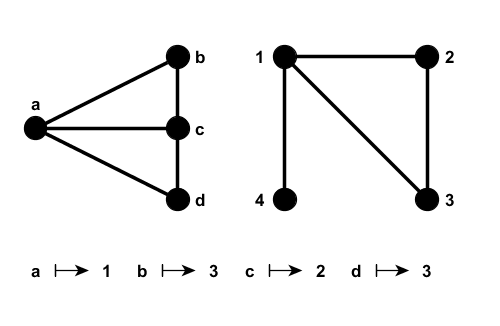
\includegraphics[width=\textwidth]{chapter1/fig/homomorphism}
        \caption{Graph homomorphism}
        \label{fig:homomorphism}
    \end{subfigure}
    \caption{Exact graph matching problems}\label{fig:Exact_GM}
\end{figure}

%\subsection{Compexity}
All problems except graph isomorphism are proofed to be $NP-$complete~\cite{Garey_NPComplet}. This can be shown through the reduction of the matching problem to the clique problem. The graph isomorphism is currently shown to be $NP-$hard~\cite{Garey_NPComplet,Schoening_GI}. For special types of graphs there exist polynomial time algorithms (e.g. for %planar graphs~\cite{Hopcroft_Wong} and 
trees~\cite{Aho_Ullman, Garey_NPComplet}).

%\subsection{Methods}
The most widespread approach to solve exact graph matching problem is branch and bound~\cite{Reingold} algorithm. It starts from some empty solution and tries in each step to expend it's current known solution based on some rules. If it happens, that a current solution does not fulfill problem's constraints, the solution is cut and algorithm backtracks to the last feasible solution and tries to expand it in other way. The most famous algorithm, that uses this principle is the one by Ullman~\cite{Ullmann}. Later it was extended and improved mostly by the suggestion of a new pruning heuristic (see for example~\cite{Lee2013} for comparison of algorithms based on the same technique).

The other techniques, that were successfully applied for the (sub)graph isomorphism are decision trees~\cite{Messmer1999,Shearer1998,Shearer2001} and group theory\cite{McKay} for maximal subgraph matching. 

\section{Inexact graph matching}

Sometimes it is difficult to apply the exact matching algorithms described in previous section to real world problems. There are two possible reasons for that. On the one hand, that are variations in the structure of graphs, that describe a same object. Those variations could be a consequence of natural deformations or noise influence, that can occur in some real word applications. On the other hand, solving the graph matching problem exactly can be time or memory consuming. As a consequence one can be interested in solving graph matching problem inexactly. In this case, no edge preserving mapping between the nodes of two graphs is required.

\begin{figure}[h!]
	\centering
	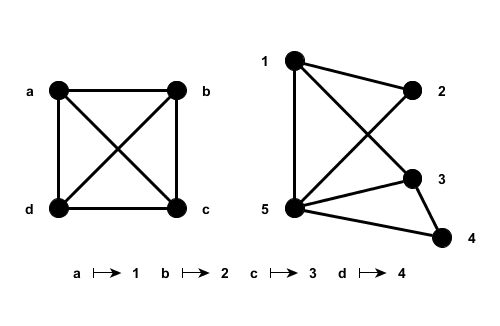
\includegraphics[width=0.5\textwidth]{chapter1/fig/inexactGM}
    \caption{Inexact graph matching}
    \label{fig:inexact_GM}
\end{figure}
    

Let us recall the problem statement \eqref{gGMP}: 
\begin{equation*}
m = \argmax_{\hat{m}}S(G^I, G^J, \hat{m})
\end{equation*}
where $S(G^I, G^J, \hat{m})$ defines the similarity measure between the attributed graphs $G^I = (V^I, E^I,D^I)$ and $G^J = (V^J, E^J,D^J)$. The mapping $m$ is required to be total and sometimes also injective, to guarantee one-to-one matching.

Depending if an algorithm for solving \eqref{gGMP} finds a global solution or not, it is called \emph{optimal} or \emph{suboptimal}. The choice, which algorithm to select depends on a specific problem. It should be noted, that an optimal inexact algorithms is not necessary faster than the exact one. On the other hand, suboptimal inexact algorithms often do not have any performance guarantee.

There are also different ways to define a similarity function $S(G^I,G^J,m)$, which leads to high number of different approaches inside the group of inexact graph matching algorithms. In the following section we summarized the most common form of objective function of the problem \eqref{gGMP}.

\subsection{Graph Matching Objective Function}

In some literature instead of defining the similarity function as in \eqref{gGMP} one speaks about dissimilarity between two graphs~\ToDo{cite} or matching score~\ToDo{cite}. The goal in this case is to minimize those values. Two versions of the problem formulation are however equivalent and one can easy transform one into other.

\subsection{Quadratic Optimization Problem}
The objective of graph matching is to find a mapping between two attributed graphs $G^I = (V^I, E^I,D^I)$ and $G^J = (V^J, E^J,D^J)$. Let the size of the graphs be $n_1$ and $n_2$ respectively. Generally, $n_1$ and $n_2$ can be different, but then we assume without losing generality $n_1\le n_2$. Here and further, we require the mapping $m$ in \eqref{gGMP} to be total and injective, which guarantees, that each node of the first graph will be matched to exactly one node of the second graph (one-to-one matching). 

We start with a even stricter assumption, that $n_1=n_2=n$ and the matching is bijective. In this case a mapping between nodes of the two graphs defines a permutation $\sigma$ of the set $\{1,\dots,n\}$. Each permutation $\sigma$ can be represented by the permutation matrix $P=\{P_{ij}\}$, where
\begin{equation*}
P_{ij}=\begin{cases}
 1, & \text{if } \sigma(i)=j, \\
 0, & \text{otherwise.} \\
\end{cases}
\end{equation*}
We denote with $\Pi_n$ the set of all feasible permutations:
\begin{equation*}
\Pi_n=\{P\in\{0,1\}^{n\times n}|\sum_{i=1,\dots,n}P_{ij}=\sum_{j=1,\dots,n}P_{ij}=1\quad\forall i,j=1,\dots,n\}
\end{equation*}
Let matrices $A^I$ and $A^J$ be the adjacency matrices of the graphs $G^I$ and $G^J$ respectively. We assume, that in case of weighed graphs, the adjacency matrices contain edge weights, instead of binary values. We can now formulate the graph matching problem as~(compare with \cite{FastPFP,Roth2001,Vogelstein_BrainGraphs}\ToDo{cite}):
\begin{equation} \label{eq:QAP1}
%P = \argmin_{\hat{P}\in\Pi_n}\|A^I\hat{P}-\hat{P}A^J\|^2
P = \argmin_{\hat{P}\in\Pi_n}\|A^I-\hat{P}A^J\hat{P}^T\|^2
\end{equation}
where $\|\cdot\|$ is the matrix Frobenius norm. After some transformations, the problem \eqref{eq:QAP1} can be reformulated as~(see~\cite{Burkard98thequadratic}, Appendix~\ref{appendixA}):
\begin{equation} \label{eq:QAP2}
P = \argmin_{\hat{P}\in\Pi_n}vec(\hat{P})^T((A^J)^T\otimes(A^I)^T)vec(\hat{P})
\end{equation}
where $\otimes$ denotes the Kronecker product and $vec(\hat{P})$ is a column-wise vectorization of $\hat{P}\in\Pi_n$.

The objective function of \eqref{eq:QAP2} is a negation of the objective of the \emph{quadratic assignment problem} with linear cost matrix set to zero, which is know to be $NP-$hard~\cite{Burkard98thequadratic,Sahni1974}. The both formulations have their advantages and disadvantages. The main benefit of \eqref{eq:QAP1} is the low space complexity $\mathcal O(n^2)$, where the space requirement of \eqref{eq:QAP2} estimates with $\mathcal O(n^4)$. This makes the second formulation tractable only for relative small graphs. The drawback of both formulations is the strict penalization function of edge disagreements, namely the squared euclidean distance between matched edges. This follows straight forward from \eqref{eq:QAP1}. In this sense the last formulation can be easily generalized in the way, we represent below. 

We return back to the case where $n_1\not=n_2$. Let denote with a binary vector $x\in \{0,1\}^{n_1n_2}$ the column-wise vectorization of the assignment matrix $P$, which is not necessary a permutation matrix anymore. It is obviously, that $x_{(j-1)n_1+i}=1$, if node $v_i\in V^I$ is matched to node $u_j\in V^J$, and $x_{(j-1)n_1+i}=0$ otherwise. For simplicity we will write further $x_{ij}$ instead of complicate $x_{(j-1)n_1+i}$.
 

%For this, we also assume, that $|V^I|=n_1$, $|V^J|=n_2$ and $n_1$ is not necessary equal to $n_2$. The maximum number of possible matches is though equal to $\min(n_1, n_2)$.

To measure a similarity between graphs one consider two different kinds of similarities: second-order \emph{edge similarity} and first-order \emph{node similarity}. The first one is defined as a function of the edges $s_E:E^I\times E^J\rightarrow\mathbb{R}$ and should penalize disagreements in the structure of two graphs. The second one $s_V:V^I\times V^J\rightarrow\mathbb{R}$ represent additional constrains on the possible node correspondences.

%Now we want to reformulate the objective function in \eqref{gGMP} using introduced node and edge similarity functions.
%A found mapping m (see Eq.~\eqref{gGMP}) gives us a set of node correspondences, which maximizes the similarity value between two graphs. Such a subset can be represented by a binary vector $x\in \{0,1\}^{n_1n_2}$, where $x_{(j-1)n_1+i}=1$, if node $v_i\in V^I$ is matched to node $u_j\in V^J$, and $x_{(j-1)n_1+i}=0$ otherwise. For simplicity we will write further $x_{ij}$ instead of $x_{(j-1)n_1+i}$.
%\footnote{Vector $x$ is a column wise vectorization of the correspondence matrix $X\in\{0,1\}^{n_1\times n_2}$, where $X_{ij}=1$, if the node $v_i\in V^I$ is matched to the node $v_j\in V^J$, and $0$ otherwise.}

Using the introduced notation and definitions of the node and edge similarity functions the function $S(G^I,G^J,m)$ in~\eqref{gGMP} can be now rewrite as follows:
\begin{equation}
	S(G^I,G^J,m)=\sum_{\substack{x_{ij}=1\\x_{i'j'}=1}}s_E(e_{ij},e_{i'j'}) + \sum_{x_{ij}=1}s_V(v_{i},v_{j})
\end{equation}
This formula can be also expressed in matrix form. We define an \emph{affinity} or \emph{similarity matrix} $A\in\mathbb{R}^{n_1n_2\times n_1n_2}$, whose diagonal elements are $s_V(v_i, u_j)$ and non-diagonal elements are $s_E(e_{ii\prime}, e_{jj\prime})$. Using this matrix we become the following formulation of the graph matching problem as an quadratic optimization problem \cite{Cho2014_Haystack, Cho2010_RRWM, Cho2012_ProgressiveGM, Conte2004}:
\begin{alignat}{2}
    &     && \argmax_x{x^TSx}                           \label{eq:gQAP1}\\ %\notag\\
    & \text{s.t. } &&  x\in \{0,1\}^{n_1n_2}            \label{eq:gQAP2}\\
    &             &&  \sum_{i=1\dots n_1} x_{ij}\le 1    \label{eq:gQAP3}\\
    &             &&  \sum_{j=1\dots n_2} x_{ij}\le 1    \label{eq:gQAP4}
\end{alignat}
We notice, that in the case, where $n_1=n_2$, both conditions (\ref{eq:gQAP3}) and (\ref{eq:gQAP4}) will be fulfilled with equality.

One can easily see, that the formulation \eqref{eq:QAP2} can be obtained from \eqref{eq:QAP1}-\eqref{eq:gQAP4} by setting $S=-(A^J)^T\otimes(A^I)^T$.
%A Quadratic Optimization Problem is known to be \emph{NP}-hard \cite{Sahni1974}. This limits greatly the size of a graph, for which a exact solution can be calculated in reasonable time. Due to this there are a number of algorithms \cite{Cho2014_Haystack, Cho2010_RRWM, Cho2012_ProgressiveGM, Chui2003, Suh_CVPR2015}, that solve graph matching problem inexact.

Below we list a different ways to define a node and edge similarities between two attributed graphs we found in the literature.
\vspace{-5pt}
\begin{itemize}
	\item Node similarity\\
	The most frequently used approach to define a node similarity is to compare attributes of the corresponding nodes. In most of seen literature, the node attributes are represented by $d-$dimensional real vector: $D^i,D^J\subset\mathbb{R}^d$. One of the simplest ways to define a node similarity in this case is to use a distance metric:
	\begin{equation}
	s_V(v_i,v_j) = dist(d_i,d_j)\text{, for }\forall v_i\in V^I,\forall v_j\in V^J
	\end{equation}
	It can be, for example, an euclidean distance %$dist_e(d_i,d_j)=\sqrt{\sum_{k=1,..d}(d^k_{i}-d^k_{j})^2}$
	(\cite{Cho2010_RRWM}\ToDo{cite}).
	The other widely used alternative to define node similarity, is to use cosine similarity\footnote{Cosine similarity is not distance metric, because it does not fulfill the triangular inequality.} of node attributes ~\cite{CliqueGraph_CVPR2015}\ToDo{cite}: $dist_c(d_i,d_j)=\frac{d_i\cdot d_j}{\|d_i\|_2\|d_j\|_2}$, where dot signifies scalar product of two vectors.
	\vspace{-5pt}
	\item Edge similarity\\
	One possible approach to calculate edge similarity is to calculate \emph{edge dissimilarity} $d_E:E^I\times E^J\rightarrow\mathbb{R}$ first and then transform it into similarity by using, for example, one of the following functions~\cite{Cho2014_Haystack, Cho2009_AgglClustering, Cho2010_RRWM,Cho2012_ProgressiveGM}:
	\begin{itemize}
		\item $s_E(e_{ii\prime}, e_{jj\prime})= exp(-\frac{d_(e_{ii\prime}, e_{jj\prime})^2}{\sigma^2_{s}})$
		\item $s_E(e_{ii\prime}, e_{jj\prime})= \max(\beta - d_(e_{ii\prime}, e_{jj\prime})/\sigma^2_{s},0)$
	\end{itemize}
	where $e_{ii\prime}\in E^I$ and $e_{jj\prime}\in E^J$. The parameters $\sigma_s$ and $\beta$ define a sensibility of a graph matching algorithm to the dissimilarities between the graphs.
	
	This leads us to the question how to calculate edge dissimilarity. The most obvious way is to compare a weights of the edges, if such are provided. An other alternative could be to use length of the edges~\cite{Cho2014_Haystack, Cho2009_AgglClustering, Cho2010_RRWM,Cho2012_ProgressiveGM}, if coordinates of the nodes in some system (usually, Cartesian coordinates) are known. It a significant assumptions, which holds however for almost all graphs arose in practical application.
	
	If the nodes of the graphs is described not only by their location, but also by some affine region around the nodes, one can use so-called geometric dissimilarity~\cite{Cho2009_AgglClustering,Cho2012_ProgressiveGM}:
	\begin{alignat}{4}
	& d(e_{ij},e_{i'j'}) && =\frac{1}{2}(d_{geo}(m_j|m_i) && +d_{geo}(m_i|m_j)) \\
	& d_{geo}(m_j|m_i) && =\frac{1}{2}(\|x_{j'}-H_{i}x_j\| && + \|x_{j}-H^{-1}_ix_{j'}\|) \\
	& d_{geo}(m_i|m_j) && =\frac{1}{2}(\|x_{i'}-H_{j}x_i\| && + \|x_{i}-H^{-1}_{j}x_{i'}\|) 
	\end{alignat}
	where $m_i$ is a correspondence between nodes $v_i$ and $v_{i'}$ and $H_i$ is a homography from $v_i$ to $v_{i'}$ defined by the provided affine regions around each node.
\end{itemize}
\vspace{-5pt}

In following we briefly describe a common approaches for solving inexact graph matching problem, used in field of Computer Vision and Pattern Recognition. We subdivided them into groups based on their main idea.

\subsection{Tree search}

\subsection{Quadratic Assignment Problem}

\subsection{Probabilistic approach}

\subsection{Spectral matching}

\subsection{Clustering matching}

\subsection{Reset algorithms for big graphs}










\section{Graph matching algorithms studied in this thesis}

\section{Discussion}